\documentclass{article}\usepackage[]{graphicx}\usepackage[]{xcolor}
% maxwidth is the original width if it is less than linewidth
% otherwise use linewidth (to make sure the graphics do not exceed the margin)
\makeatletter
\def\maxwidth{ %
  \ifdim\Gin@nat@width>\linewidth
    \linewidth
  \else
    \Gin@nat@width
  \fi
}
\makeatother

\definecolor{fgcolor}{rgb}{0.345, 0.345, 0.345}
\newcommand{\hlnum}[1]{\textcolor[rgb]{0.686,0.059,0.569}{#1}}%
\newcommand{\hlstr}[1]{\textcolor[rgb]{0.192,0.494,0.8}{#1}}%
\newcommand{\hlcom}[1]{\textcolor[rgb]{0.678,0.584,0.686}{\textit{#1}}}%
\newcommand{\hlopt}[1]{\textcolor[rgb]{0,0,0}{#1}}%
\newcommand{\hlstd}[1]{\textcolor[rgb]{0.345,0.345,0.345}{#1}}%
\newcommand{\hlkwa}[1]{\textcolor[rgb]{0.161,0.373,0.58}{\textbf{#1}}}%
\newcommand{\hlkwb}[1]{\textcolor[rgb]{0.69,0.353,0.396}{#1}}%
\newcommand{\hlkwc}[1]{\textcolor[rgb]{0.333,0.667,0.333}{#1}}%
\newcommand{\hlkwd}[1]{\textcolor[rgb]{0.737,0.353,0.396}{\textbf{#1}}}%
\let\hlipl\hlkwb

\usepackage{framed}
\makeatletter
\newenvironment{kframe}{%
 \def\at@end@of@kframe{}%
 \ifinner\ifhmode%
  \def\at@end@of@kframe{\end{minipage}}%
  \begin{minipage}{\columnwidth}%
 \fi\fi%
 \def\FrameCommand##1{\hskip\@totalleftmargin \hskip-\fboxsep
 \colorbox{shadecolor}{##1}\hskip-\fboxsep
     % There is no \\@totalrightmargin, so:
     \hskip-\linewidth \hskip-\@totalleftmargin \hskip\columnwidth}%
 \MakeFramed {\advance\hsize-\width
   \@totalleftmargin\z@ \linewidth\hsize
   \@setminipage}}%
 {\par\unskip\endMakeFramed%
 \at@end@of@kframe}
\makeatother

\definecolor{shadecolor}{rgb}{.97, .97, .97}
\definecolor{messagecolor}{rgb}{0, 0, 0}
\definecolor{warningcolor}{rgb}{1, 0, 1}
\definecolor{errorcolor}{rgb}{1, 0, 0}
\newenvironment{knitrout}{}{} % an empty environment to be redefined in TeX

\usepackage{alltt}
% \usepackage[backend = biber, style=numeric]{biblatex}
\usepackage[backend = bibtex, style=numeric]{biblatex}


\bibliography{bibliography}
\usepackage{pdfpages}

\usepackage{indentfirst}
\usepackage{todonotes}
\usepackage{listings}
% \addbibresource{bibliography.bib}
% \usepackage{lipsum}
\usepackage{hyperref}
\usepackage[a4paper, portrait, margin=1in]{geometry}
\usepackage{setspace}
\setstretch{1.25}
\hypersetup{
    linkcolor=blue
    colorlinks=true,
    citecolor=magenta,      
    urlcolor=cyan,
}
\usepackage{parskip}
\usepackage{graphicx}
\usepackage{amsmath}
\usepackage{amsthm}
\usepackage{amssymb}
\usepackage{setspace}
\usepackage{parskip}
\usepackage{bbm}

\theoremstyle{plain}
\newtheorem{theorem}{Theorem}[section]
\newtheorem{lemma}[theorem]{Lemma}
\newtheorem{corollary}[theorem]{Corollary}
\newtheorem{observation}[theorem]{Observation}
\newtheorem{proposition}[theorem]{Proposition}

\theoremstyle{definition}
\newtheorem{definition}[theorem]{Definition}{}{}
\newtheorem{problem}[theorem]{Problem}
\newtheorem{assumption}[theorem]{Assumption}
\newtheorem{example}[theorem]{Example}


\theoremstyle{remark}
\newtheorem{claim}[theorem]{Claim}
\newtheorem{remark}[theorem]{Remark}

\newcommand{\boldY}{\mathbf{Y}}
\newcommand{\boldZ}{\mathbf{Z}}
\newcommand{\boldz}{\mathbf{z}}
\newcommand{\boldy}{\mathbf{y}}
\newcommand{\boldx}{\mathbf{x}}
\newcommand{\boldtheta}{\boldsymbol{\theta}}
\newcommand{\boldPsi}{\boldsymbol{\Psi}}
\newcommand{\boldxi}{\boldsymbol{\xi}}
\newcommand{\boldtau}{\boldsymbol{\tau}}
\newcommand{\boldmu}{\boldsymbol{\mu}}
\newcommand{\boldSigma}{\boldsymbol{\Sigma}}
\newcommand{\boldOmega}{\boldsymbol{\Omega}}
\DeclareMathOperator*{\argmax}{\arg\!\max}

\title{\textbf{A Practical Introduction to Finite Mixture Models in R} \\ [.6cm] \normalsize Semester Paper}

\author{Wayne Zeng\\[.6cm]{Supervisor: Dr. Lukas Meier} \\[2cm] \normalsize Seminar for Statistics \\ \normalsize D-MATH \\ \normalsize ETH Zurich}

\date{\normalsize Spring Semester 2022}
\IfFileExists{upquote.sty}{\usepackage{upquote}}{}
\begin{document}
\maketitle
\vspace{2em}
\begin{abstract}
Finite mixture models are a flexible and convenient way to model unknown distributional shapes. They are also good at modelling group structures. A gentle introduction to mixture models will be given, as well as practical use cases in \texttt{R}, covering the package \texttt{mixtools}.
\end{abstract}

\newpage

{
  \hypersetup{linkcolor=blue}
  \tableofcontents
}

\newpage
%%%%%%%%%%%%%%%%%%%%%%%%%%%%%%%%%%%%%%%%%%%%%%%%%%%%%%%%%%%%%%%%%%%%%%%%%%%%%%%%%%%%%%%%%%%%%%%%%%%%%%%%%%%%%%%%%%%%%%%%%%%%%%%%%%%%%%%%%%%%%%%%%%%%%%%%%%%%%%%%%%%


\section*{Introduction}

Classification and subgrouping are important in many fields of data analysis. In many datasets, the memberships of each datapoint may not be easily discernible. The basic goal in such cases is to examine a sample of measurements and to differentiate these subgroups of individuals, even when there are no observable variables that readily indicate which subgroup an individual properly belongs. This leads to notions such as model-based clustering and unsupervised clustering.

Finite mixtures of distributions, a.k.a. \textit{finite mixture models} or FMMs, are used to provide computationally convenient representations for modelling complex distributions of data on random phenomena. FMMs form the bases of cluster and latent class analyses, discriminant analysis and image analysis. They also provide descriptive models for distributions where a single component distribution is insufficient, i.e. they can give descriptions of entire subgroups, rather than assignments of individuals to those subgroups.

In \hyperref[sec:formulation]{Section 1}, we introduce the definition of a finite mixture model. \hyperref[sec:EM]{Section 2} explores latent variable models and the EM Algorithm as an alternative to maximum likelihood estimation. \hyperref[sec:GMM]{Section 3} then introduces the most commonly used FMM, the Gaussian Mixture Model, and lastly \hyperref[sec:Iris]{Section 4} applies the above to the Iris Dataset in \texttt{R}.

Much of Sections 1--3 closely follows McLachlan and Peel's ``Finite Mixture Models'' \cite{FMMs_Book}.

\section*{Acknowledgements}

I would like to thank my supervisor, Lukas Meier, for his support and patience over the last few months. The fast, precise communication we were able to maintain was invaluable for my progress and understanding throughout the writing of this paper, and is greatly appreciated.

\newpage

%%%%%%%%%%%%%%%%%%%%%%%%%%%%%%%%%%%%%%%%%%%%%%%%%%%%%%%%%%%%%%%%%%%%%%%%%%%%%%%%%%%%%%%%%%%%%%%%%%%%%%%%%%%%%%%%%%%%%%%%%%%%%%%%%%%%%%%%%%%%%%%%%%%%%%%%%%%%%%%%%%%
%%%%%%%%%%%%%%%%%%%%%%%%%%%%%%%%%%%%%%%%%%%%%%%%%%%%%%%%%%%%%%%%%%%%%%%%%%%%%%%%%%%%%%%%%%%%%%%%%%%%%%%%%%%%%%%%%%%%%%%%%%%%%%%%%%%%%%%%%%%%%%%%%%%%%%%%%%%%%%%%%%%
\section{Formulation of Mixture Distributions} \label{sec:formulation}
\subsection{Basic Definition}
Let $\boldY_1, \dots, \boldY_n$ denote a random sample of size $n \geq 1$, where $\boldY_j$ is a $p$-dimensional random vector with probability density function (pdf) $ f(\mathbf{y}_j)$ on $\mathbb{R}^p$. The vector $\boldY_j$ contains the random variables corresponding to $p$ measurements    
\begin{definition} \label{def:FMM1}
    The probability density function (pdf), or in the discrete case, the probability mass function, of a $p$-dimensional random vector $\mathbf{Y}$ takes the form
    \begin{equation} \label{def:mixdistr1}
        f(\mathbf{y}) = \sum_{i=1}^g \pi_i f_i(\mathbf{y}),
    \end{equation}
\end{definition}
where the coefficients or ``mixing proportions'' $\pi_i$ are non-negative and $\sum_{i=1}^g \pi_i = 1$, and $f_i(\mathbf{y})$ are the $g-$component densities, where $g \geq 1$ denotes the number of components in the mixture model.

The component densities may be parameterised with a vector $\boldtheta_i$ of parameters. We can then rewrite the above definition \eqref{def:FMM1} as
\begin{equation} \label{def:parmix}
    f(\mathbf{y}; \mathbf{\Psi}) = \sum_{i=1}^g \pi_i f_i(\boldy ; \boldtheta_i),
\end{equation}
where $\boldPsi = (\pi_1, \pi_2, \dots, \pi_{g-1}, \boldxi^T)$ is the vector of unknown parameters and $\boldxi$ is the vector containing all the parameters in $\boldtheta_1, \dots, \boldtheta_g$ known in advance to be distinct.

\subsection{Interpretation of Mixture Models}

We can generate a random vector $\boldY$ with $g$-component mixture density \eqref{def:mixdistr1} by defining a new categorical random variable $Z_j$ such that:
\begin{gather*}
    Z_j = \{1, \dots, g\}, \\
    P(Z_j = i) = \pi_i, \\
    P(\boldY_j \vert Z_j = i) = f(\boldy).
\end{gather*}
Then the marginal density of $\boldY$ is precisely $f(\boldy)$.

We will see in \hyperref[subsec:incomplete]{Subsection 2.2.1} that it is convenient to work with a $g$-dimensional label.

\subsection{Example: Mixtures of Two Normal Homoscedastic Components}

Consider a mixture of two univariate normal components with common variance $\sigma^2$ and means $\mu_1, \mu_2$ with corresponding mixture proportions $\pi_1, \pi_2$ such that
\begin{equation} \label{ex:homomix}
    f(y_i) = \pi_1 \phi(y_j; \mu_1, \sigma^2) + \pi_2 \phi(y_j; \mu_2, \sigma^2), \qquad \phi(y_j; \mu_i, \sigma^2) = \frac{1}{\sigma \sqrt{2 \pi}} e^{-\frac{(y_j - \mu_j)^2}{2 \sigma^2}}.
\end{equation}

We consider two scenarios: one where the means of the two component normal densities are far apart vs. when they are sufficiently close together. If the two means are far apart, then we would expect \eqref{ex:homomix} to resemble two normal densities side by side. For this purpose, let us define the Mahalanobis distance:
\nopagebreak
\begin{equation*}
    \Delta = \vert \mu_1 - \mu_2 \vert / \sigma
\end{equation*}

In the other case where the means are more closely together, it is more difficult to see the distinction between them, leading to an asymmetric density if the components are not represented in equal proportions.

We now generate our first mixture model. Below is an example in \texttt{R} where we sum Gaussian components, each with means further away from each other than the last.

\begin{minipage}{\linewidth}
\singlespacing
\begin{knitrout}
\definecolor{shadecolor}{rgb}{0.969, 0.969, 0.969}\color{fgcolor}\begin{kframe}
\begin{alltt}
\hlkwd{set.seed}\hlstd{(}\hlnum{123}\hlstd{)}
\hlkwd{par}\hlstd{(}\hlkwc{mfrow}\hlstd{=}\hlkwd{c}\hlstd{(}\hlnum{2}\hlstd{,}\hlnum{2}\hlstd{))}
\hlstd{x} \hlkwb{<-} \hlkwd{seq}\hlstd{(}\hlopt{-}\hlnum{10}\hlstd{,} \hlnum{10}\hlstd{,} \hlkwc{length}\hlstd{=}\hlnum{100}\hlstd{)}
\hlstd{y} \hlkwb{<-} \hlnum{.5} \hlopt{*} \hlstd{(}\hlkwd{dnorm}\hlstd{(x)} \hlopt{+} \hlkwd{dnorm}\hlstd{(x,} \hlkwc{mean}\hlstd{=}\hlnum{1}\hlstd{))}
\hlstd{y0} \hlkwb{<-} \hlnum{.5} \hlopt{*} \hlstd{(}\hlkwd{dnorm}\hlstd{(x)} \hlopt{+} \hlkwd{dnorm}\hlstd{(x,} \hlkwc{mean}\hlstd{=}\hlnum{2}\hlstd{))}
\hlstd{y1} \hlkwb{<-} \hlnum{.5} \hlopt{*} \hlstd{(}\hlkwd{dnorm}\hlstd{(x)} \hlopt{+} \hlkwd{dnorm}\hlstd{(x,} \hlkwc{mean}\hlstd{=}\hlnum{3}\hlstd{))}
\hlstd{y2} \hlkwb{<-} \hlnum{.5} \hlopt{*} \hlstd{(}\hlkwd{dnorm}\hlstd{(x)} \hlopt{+} \hlkwd{dnorm}\hlstd{(x,} \hlkwc{mean}\hlstd{=}\hlnum{5}\hlstd{))}
\hlkwd{plot}\hlstd{(x, y,} \hlkwc{type}\hlstd{=}\hlstr{"l"}\hlstd{,} \hlkwc{main}\hlstd{=}\hlstr{".5 * (N(0,1)+N(1,1))"}\hlstd{)}
\hlkwd{plot}\hlstd{(x, y0,} \hlkwc{type}\hlstd{=}\hlstr{"l"}\hlstd{,} \hlkwc{main}\hlstd{=}\hlstr{".5 * (N(0,1)+N(2,1))"}\hlstd{)}
\hlkwd{plot}\hlstd{(x, y1,} \hlkwc{type}\hlstd{=}\hlstr{"l"}\hlstd{,} \hlkwc{main}\hlstd{=}\hlstr{".5 * (N(0,1)+N(3,1))"}\hlstd{)}
\hlkwd{plot}\hlstd{(x, y2,} \hlkwc{type}\hlstd{=}\hlstr{"l"}\hlstd{,} \hlkwc{main}\hlstd{=}\hlstr{".5 * (N(0,1)+N(5,1))"}\hlstd{)}
\end{alltt}
\end{kframe}

{\centering 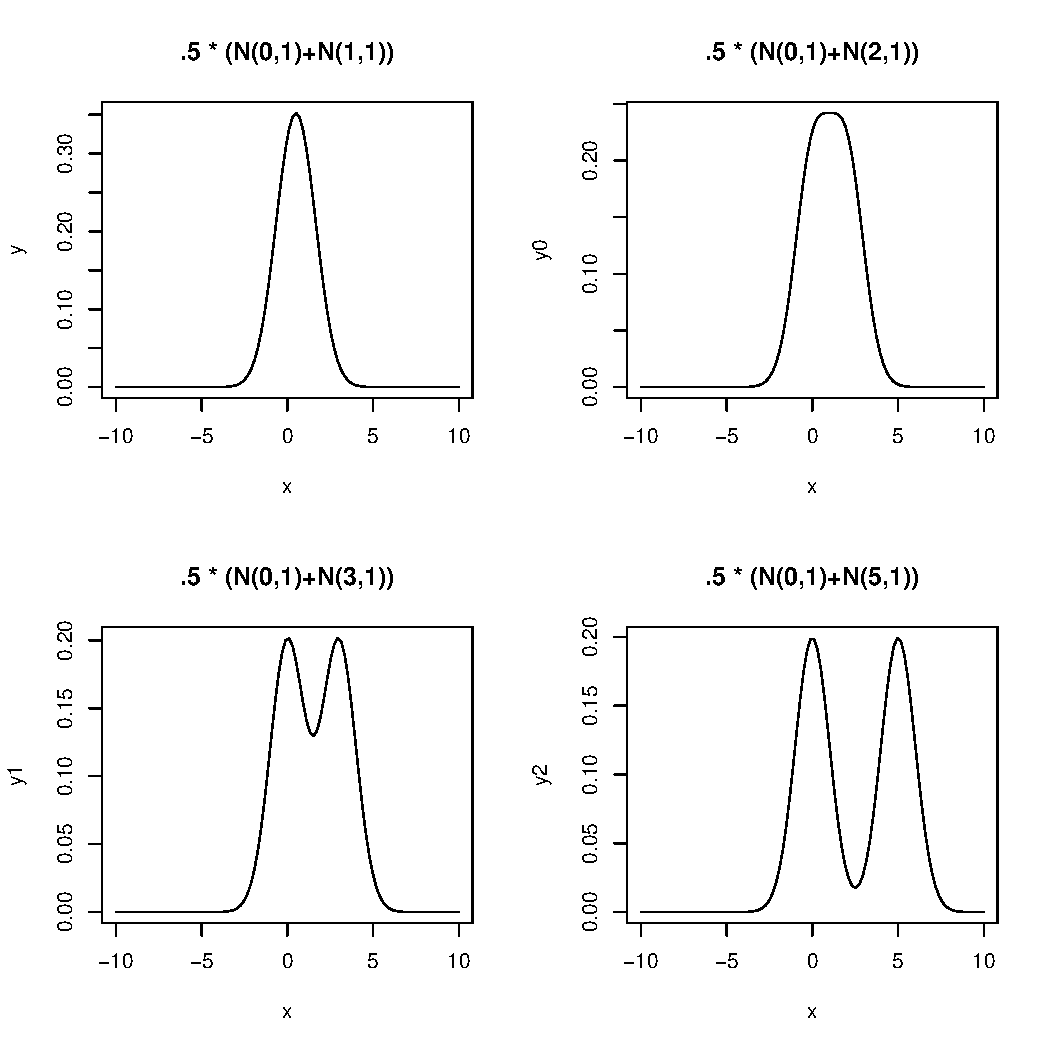
\includegraphics[width=4in]{figure/myrcode0-1} 

}


\end{knitrout}
\end{minipage}

\subsection{Parametric Models}

We will mostly be focusing on parametric mixture models. These models have the component densities $f_i(\boldy_j)$ belonging to some parametric family $\boldtheta_i$. We can then rewrite this as $f_i(\boldy_i; \boldtheta_i)$,   $\boldtheta_i$ being the vector of unknown parameters in the postulated form for the $i$th component density in the mixture.

We rewrite \eqref{ex:homomix} as
\begin{equation*}
    f(\boldy_j ; \boldPsi) = \sum_{i=1}^g \pi_i f_i(\boldy_j; \boldtheta_j), \quad  \boldPsi = (\pi_1, \dots, \pi_{g-1}, \boldxi^T)^T
\end{equation*}


\subsection{Identifiablity and Component Labels}
Based on \cite[Section 2.2]{annurev_FMMs}.

For parametric families, $f(\boldy; \boldPsi)$ is \textit{identifiable} if the distinct values of $\boldPsi$ determine distinct members of $\{f(\boldy; \boldPsi): \, \boldPsi \in \boldOmega\}$, where $\boldOmega$ is the parameter space. However, the mixture distribution definition is slightly different:
\begin{definition}
  Let $f(\boldy; \boldPsi) = \sum_{i=1}^g \pi_i f_i(\boldy; \boldtheta_i)$ and $f(\boldy; \boldPsi^*) = \sum_{i=1}^{g^*} \pi_i^* f_i(\boldy; \boldtheta_i^*)$ be two arbitrary members of a parametric family of mixture densities. Then this class of mixtures is \textit{identifiable} for $\boldPsi \in \boldOmega$ if $f(\boldy; \boldPsi) \equiv f(\boldy; \boldPsi^*) \iff g = g^*$.
\end{definition}
Intuitively, this means that we can permute the component labels so that $\pi_i = \pi_i^*$ and $f_i(\boldy; \boldtheta_i) = f_i(\boldy; \boldtheta_i^*)$, and that $f(\boldy; \boldPsi)$ is invariant under the $g!$ permutations of said component labels.

In practice, a lack of identifiablity can be easily mitigated by, for example, imposing conditions on $\boldPsi$ so that $\pi_1 \leq \pi_2 \leq \dots \leq \pi_g$. However, issues then arise when we consider a Bayesian framework where posterior simulation is used to make inferences from the mixture model (also known as label-switching problem).

\newpage

%%%%%%%%%%%%%%%%%%%%%%%%%%%%%%%%%%%%%%%%%%%%%%%%%%%%%%%%%%%%%%%%%%%%%%%%%%%%%%%%%%%%%%%%%%%%%%%%%%%%%%%%%%%%%%%%%%%%%%%%%%%%%%%%%%%%%%%%%%%%%%%%%%%%%%%%%%%%%%%%%%%
%%%%%%%%%%%%%%%%%%%%%%%%%%%%%%%%%%%%%%%%%%%%%%%%%%%%%%%%%%%%%%%%%%%%%%%%%%%%%%%%%%%%%%%%%%%%%%%%%%%%%%%%%%%%%%%%%%%%%%%%%%%%%%%%%%%%%%%%%%%%%%%%%%%%%%%%%%%%%%%%%%%


\section{Maximum Likelihood Fitting of Mixture Models and the EM Algorithm}\label{sec:EM}
Loosely based on \cite{EM_Info}.

Maximum likelihood estimation (MLE) is the most commonly used approach to fitting mixture distributions and density estimation. This is done by searching across probability distributions and their parameters. However, MLE requires our dataset to be complete, since the likelihood no longer can be factorised and nor is it convex anymore, leading to a lack of a closed solution whilst maximising said likelihood. Furthermore, Bayesian inference of the parameters is made harder.

The \textit{Expectation Maximisation Algorithm}, or EM, is used to perform MLE in the presence of latent variables. This is a general algorithm commonly used for density estimation with missing/latent data.

The EM algorithm is an iterative approach that cycles between two steps:
\begin{enumerate}
    \item The first E-step (expectation) attempts to estimate the missing or latent variables.
    \item The second M-step (maximisation) optimises the parameters of the model to explain the data.
\end{enumerate}
We repeat this process until we reach convergence.

\subsection{Latent Variable Models and Relationship to FMMs}

In many statistical problems, there are many variables which cannot be measured directly. We denote these variables to be \textit{latent}. We often link these latent variables to observable ones in order to infer the values of the latent ones.

Usually, statistical procedures and learning algorithms are used to estimate parameters of probability distributions to best fit the density of a given training dataset, mostly using maximum likelihood.

Let us consider the most simple case of a finite mixture model, where the dataset is comprised of many points that happen to be generated by two different processes. We generate the points to be Gaussian distributed, but the distributions are similar enough that it is not obvious to which distribution a given point may belong. The important remark here is that processes used to generate such data \textit{represents} our latent variables. This clearly influences the data, but is not observable. As seen above, we cannot simply use MLE anymore, thus EM can be employed to estimate the parameters of a FMM.

\subsection{Application of the EM Algorithm}

\subsubsection{Formulation as Incomplete Data Problem} \label{subsec:incomplete}

We use the component label vector $\boldZ_j$ with the indicator variables. This notation is useful (although unintuitive at first) because it allows the MLE of the mixture distribution to be computed easily via the EM-algorithm. 

We write
\begin{equation*}
    \boldY_1, \dots, \boldY_n   \stackrel{i.i.d.}{\sim} F,
\end{equation*}
where $F(\boldy_i)$ denotes the distribution function corresponding to the mixture density $f(\boldy_i)$.

The feature data $\boldy_1, \dots, \boldy_n$ is incomplete since their associated component-indicator vectors $\boldz_1, \dots, \boldz_n$ are not available, hence we consider this to be a latent variable model.

Furthermore, we define the complete data vector:
\begin{equation} \label{eq:ycomplete}
    \boldy_c = (\boldy^T, \boldz^T)^T,
\end{equation}
where
\begin{equation*}
    \boldy = (\boldy_1^T, \dots, \boldy_n^T)^T \quad \boldz = (\boldz_1^T, \dots, \boldz_n^T)^T
\end{equation*}

All  the observations $\boldy_j$ have been completely recorded and fully observed. In addition, the component label vectors $\boldz$ are taken to be the realised values of the random vectors $\boldZ_1, \dots, \boldZ_n$

We can assume they are distributed unconditionally as
\begin{equation*}
    \boldZ_1, \dots, \boldZ_1, \stackrel{i.i.d.}{\sim} \text{Mult}_g (1, \boldsymbol{\pi}).
\end{equation*}

The $i$th mixing proportion $\pi_i$ can be interpreted as the prior probability that the entity belongs to the $i$th component of the mixture distribution, whereas the posterior probability that the entity belongs to the $i$th component with $\boldy_j$ having been observed on it is given by
\begin{align*}
    \tau(\boldy_j) &= P(\text{entity} \in i\text{th component } \vert \, \boldy_j ) \\
    &= P(Z_{ij} = 1 \, \vert \, \boldy_j) \\
    &= \pi_i f_i(\boldy_j) / f(\boldy_j)
\end{align*}
% Mixture model arises in incomplete-data context because component-label $\boldz_j$ are missing from complete-data vector.

This assumption means that the distribution of the complete data vector $\boldY_c$ implies the appropriate distribution for the incomplete-data vector $\boldY$. The final complete log likelihood for $\boldPsi$ is
\begin{equation} \label{eq:llcomplete}
    \log L_c (\boldPsi) = \sum_{i=1}^g \sum_{j=1}^n z_{ij} \{ \log \pi_i + \log f_i (\boldy_j ; \boldtheta_i)\}.
\end{equation}


\subsubsection{EM Algorithm}
Based on \cite[Section 2.8]{FMMs_Book}.

Let us consider the standard FMM expression:

\begin{equation*}
    f(\boldy_j ; \boldPsi) = \sum_{i=1}^g \pi_i f_i (\boldy_j ; \boldtheta_i),
\end{equation*}

Where $\boldy = (\boldy_1^T, \dots, \boldy_n^T)^T$, $\boldPsi$ is the observed incomplete data vector as defined above.

The log likelihood for $\boldPsi$ formed \textit{from the observed data is} given by the sum of the $f(\boldy_j ; \boldPsi)$s:
\begin{align*}
    \log L(\boldPsi) &= \sum_{j=1}^n \log f(\boldy_j ; \boldPsi) \\
    &=  \sum_{j=1}^n \log \{ \sum_{i=1}^g \pi_i f_i (\boldy_j ; \boldtheta_i) \},
\end{align*}
and noting the difference between this expression and \eqref{eq:llcomplete}.
To obtain the MLE, we would like to solve the likelihood equation 
\begin{equation*}
    \frac{\partial \log L(\boldPsi)}{\partial \boldPsi} = \textbf{0}. 
\end{equation*}

We denote the $\hat{\boldPsi}$ as the MLE of $\boldPsi$ and let
\begin{equation} \label{eq:EMtau}
    \tau_i (\boldy_i ; \boldPsi) = \frac{\pi_i f_i (\boldy_i;\boldtheta_i)}{\sum_{h=1}^g \pi_h f_h (\boldy_i;\boldtheta_h))}
\end{equation}
be the posterior probability that $\boldy_j$ belongs to the $i$th component of the mixture. % \todo{find original text and reference!} 
Then $\hat{\boldPsi}$ satisfies the following expressions:
\begin{equation} \label{eq:EM1}
    \hat{\pi_i} = \sum_{j=1}^n \tau_i (\boldy_i ; \hat{\boldPsi}) / n \quad (i = 1, \dots, g)
\end{equation}
and
\begin{equation} \label{eq:EM2}
    \sum_{i=1}^g \sum_{j=1}^n \tau_i (\boldy_i ; \hat{\boldPsi})  \partial \log_i (\boldy_i;\hat{\boldtheta}_i) / \partial \boldxi = \textbf{0}.
\end{equation}

The two equations \eqref{eq:EM1} and \eqref{eq:EM2} build the iterative foundation of the EM algorithm. The proof of the two above equations involves Bayes' equation and can be found in \cite[Section 1.4]{EM_Book}.

\subsubsection*{E-Step: Computing $Q(\boldPsi; \boldPsi^{(k)})$}
The E-step treats the latent data labels $\boldz_{ij}$s as missing. It handles the addition of these unobservable labels by taking the conditional expectation of the \textit{complete} log-likelihood $\log L_c (\boldPsi)$ given $\boldy$ using the current fit for $\boldPsi$. For the first step, we take this initial fit to be $\boldPsi^{(0)}$. This initial value can be found by plugging into the right hand side of the equations.
\begin{equation} \label{eq:EMFirstStep}
Q(\boldPsi; \boldPsi^{(0)}) = E_{\boldPsi^{(0)}} \{\log L_c{(\boldPsi)} \vert \boldy\}.
\end{equation}

The subscript $\boldPsi^{(0)}$ on the right hand side explicitly expresses that we are taking the expectation with respect to the current estimate $\boldPsi^{(0)}$. In later iterations, we compute a new estimate for  $\boldPsi^{(k+1)}$ by taking the expectation w.r.t. $\boldPsi^{(k)}$. 

From \eqref{eq:llcomplete}, we see that $\log L_c(\boldPsi)$ is linear in the unobservable labels $z_{ij}$. This implies that
\begin{align*}
  E_{\boldPsi^{(k)}} \{ Z_{ij} \vert \boldy\} &= \mathrm{pr}_{\boldPsi^{(k)}} \{Z_{ij} = 1 \vert \boldy \} \\
  &= \tau_i (\boldy_i ; \boldPsi^{(k)}) \\
  &= \frac{\pi_i^{(k)} f_i (\boldy_i;\boldtheta_i^{(k)})}{f(\boldy_j ; \boldPsi^{(k)})} \\
  &= \frac{\pi_i^{(k)} f_i (\boldy_i;\boldtheta_i^{(k)})}{\sum_{h=1}^g \pi_h^{(k)} f_h (\boldy_i;\boldtheta_h^{(k)}))}
\end{align*}
for $i=1, \dots, g; \, j=1, \dots, n$ in a similar fashion to \eqref{eq:EMtau}.

Substituting this expression into \eqref{eq:EMFirstStep}, we obtain the final expression for the E-step:
\begin{equation} \label{eq:EStep}
  Q(\boldPsi; \boldPsi^{(k)}) =  \sum_{i=1}^g \sum_{j=1}^n \tau_i (\boldy_i ; \boldPsi^{(k)}) \{ \log \pi_i + \log f_i (\boldy_j ; \boldtheta_i)\}.
\end{equation}

\subsubsection*{M-step: Maximising $Q(\boldPsi; \boldPsi^{(k)})$}

The aim of the M-step is to globally maximise $Q(\boldPsi; \boldPsi^{(k)})$ w.r.t. $\boldPsi$ over the parameter space $\Omega$ to produce the updated estimate $\boldPsi^{(k+1)}$. Moreover, the mixture coefficients $\pi_i^{(k+1)}$ are calculated independently from $\boldxi^{(k+1)}$.

Returning to the hypothetical case where the component labels $z_{ij}$ would be observable. Then the MLE of $\pi_i$ would be
\begin{equation}\label{eq:obsMLEpi}
  \hat{\pi}_i = \sum_{j=1}^n z_{ij} / n.
\end{equation}
In the E-step, we replaced each instance of $z_{ij}$ with its current conditional expectation $\tau_i (\boldy_i ; \boldPsi^{(k)})$ in the complete data log-likelihood. In an analogous fashion, we can transform \eqref{eq:obsMLEpi}:

\begin{equation}\label{eq:MStep1}
  \pi_i^{(k+1)} = \sum_{j=1}^n \tau_i (\boldy_i ; \boldPsi^{(k)}) / n.
\end{equation}

This substitution is intuitively significant, since we see that each currently assessed posterior probability of membership $\pi_i^{(k+1)}$ contains a contribution from each observed component $\boldy_i$ in the mixture model. As for the parameter vector $\boldxi$, we can take the partial derivative of the equation \eqref{eq:EStep} and take one of the roots:

\begin{equation}\label{eq:MStep2}
  \sum_{i=1}^g \sum_{j=1}^n \tau_i (\boldy_i ; \boldPsi^{(k)}) \partial \log f_i (\boldy_j ; \boldtheta_i) / \partial \boldxi = 0.
\end{equation}
This begs the question of whether the above equation has a closed form solution, since the original problem did not. In many cases, such as in a Gaussian mixture model, we do mostly have closed form solutions.

We cycle through the E-Step and M-step until we reach convergence, i.e.
\begin{equation*}
  L(\boldPsi^{k+1}) - L(\boldPsi^{k}) \leq \varepsilon, \, \varepsilon \text{ is usually set to } 1e-6
\end{equation*}
Furthermore, it was shown that the likelihood function is increasing after each EM iteration, i.e.
\begin{equation}
  L(\boldPsi^{k+1}) \geq L(\boldPsi^{k}).
\end{equation}


\subsection{Starting Values and Initial Parameters}\label{subsec:start}
Based on\cite[Sections 2.10, 2.12]{FMMs_Book}.

The EM algorithm requires an initial estimate of $\boldPsi^{(0)}$. A good or bad initial estimate can affect the speed of convergence of the algorithm greatly. This is especially the case if the likelihood $L_c(\boldPsi)$ is unbounded on the edge of the parameter space $\Omega$, potentially causing estimates for the $\boldPsi^{(k)}$'s to be diverge if the initial value is chosen too closely to the aforementioned boundary. Further discussion  of starting values can be found in \cite[Section 3.8]{FMMs_Book}.

In addition, the likelihood equation \eqref{eq:EM2} may possess multiple roots, prompting the use of multiple starting points in order to find all possible local maxima. In the case that there are no suitable roots, we choose the root with the largest MLE out of all the maxima.
\newpage
A random approach may also be used to specifying initial values. In the Gaussian case with $g$ normal components with means $\boldmu_i$ and covariance matrices $\boldSigma_i$, we can randomly generate the starting means $\boldmu_i^{(0)}$ as
\begin{equation*}
  \boldmu_1^{(0)}, \dots, \boldmu_g^{(0)} \stackrel{i.i.d.}{\sim} N(\bar{\boldy}, \boldsymbol{V}),
\end{equation*}
where $\bar{\boldy}$ denotes the sample mean and $\boldsymbol{V}$ the sample covariance of the observed data. Using this expression, we can specify $\boldSigma_i$ and the mixing proportions $\pi_i$ as
\begin{equation*}
  \boldSigma_i = \boldsymbol{V}, \qquad \pi_i^{(0)} = 1/g, \qquad i = 1, \dots, g.
\end{equation*}
This method provides good variation between the initial values $\boldmu_i^{(0)}$ and is not as computationally demanding as other random start methods.

However, in practice, basic clustering algorithms such as $k$-means can be employed as a way of finding starting points, as we will see in \hyperref[sec:Iris]{Section 4}.


\newpage

%%%%%%%%%%%%%%%%%%%%%%%%%%%%%%%%%%%%%%%%%%%%%%%%%%%%%%%%%%%%%%%%%%%%%%%%%%%%%%%%%%%%%%%%%%%%%%%%%%%%%%%%%%%%%%%%%%%%%%%%%%%%%%%%%%%%%%%%%%%%%%%%%%%%%%%%%%%%%%%%%%%
%%%%%%%%%%%%%%%%%%%%%%%%%%%%%%%%%%%%%%%%%%%%%%%%%%%%%%%%%%%%%%%%%%%%%%%%%%%%%%%%%%%%%%%%%%%%%%%%%%%%%%%%%%%%%%%%%%%%%%%%%%%%%%%%%%%%%%%%%%%%%%%%%%%%%%%%%%%%%%%%%%%

\section{Gaussian and Other Mixture Models}\label{sec:GMM}

This section is loosely based on \cite[Sections 3.2 and 3.3]{FMMs_Book}.

The most common case of FMMs is where all of the mixture components are multivariate Gaussian. In the context of clustering, it is appropriate to use Gaussian mixture models (GMMs) whenever the clusters appear to have elliptical or symmetric structures. Any non-normal features in the data can then be easily identified and signal some other underlying group structure. Multivariate normal distributions are relatively simple and also make the M-step of the EM algorithm easier to compute. For clusters with heavier tails, we can also consider t-tailed mixture models.

\subsection{Heteroscedastic Components}

The original FMM equation \eqref{def:parmix} expressed with Gaussian mixture components takes the form
\begin{equation} \label{def:GMM} 
  f(\boldy_j; \boldPsi) = \sum_{i=1}^g \pi_i \phi (\boldy ; \boldmu_i, \boldSigma_i),
\end{equation}
Note that $\boldxi$ in the above case is comprised of the component means $\boldmu_i$ and component covariance matrices $\boldSigma_i$, known in the heteroscedastic case to be distinct without restrictions.

The EM-Algorithm for GMMs is modified in the following way:

E-step: We modify $\tau_i (\boldy_i ; \boldPsi)$
\begin{equation}\label{eq:EStepGMM}
   \tau_i (\boldy_i ; \boldPsi) = \frac{\pi_i \phi (\boldy ; \boldmu_i, \boldSigma_i)}{\sum_{h=1}^g \pi_h \phi (\boldy ; \boldmu_i, \boldSigma_i)}, \quad i = 1, \dots, g, \quad  j = 1, \dots, n
\end{equation}

M-step: the $\pi_i$s are defined identically to the normal FMMs, see equation \eqref{eq:MStep1}.

For $\boldmu_i^{(k+1)}$ and $\boldSigma_i^{(k+1)}$ let us define the following notation:
\begin{equation} \label{eq:tauGMM}
  \tau_{ij}^{(k)} = \tau_i(\boldy_j; \boldPsi^{(k)}), \quad i = 1, \dots, g, \quad  j = 1, \dots, n.
\end{equation}
With this notation and using equation \eqref{eq:MStep2}, replacing every $f$ with $\phi$, we obtain the following:
\begin{equation} \label{eq:Mstep2GMM}
  \boldmu_i^{(k+1)} = \sum_{j=1}^n \tau_{ij}^{(k)} \boldy_j / \sum_{j=1}^n \tau_{ij}^{(k)}, \quad \quad \boldSigma_i^{(k+1)} = \sum_{j=1}^n \tau_{ij}^{(k)} (\boldy_j - \boldmu_i^{(k+1)}) (\boldy_j - \boldmu_i^{(k+1)})^T / \sum_{j=1}^n \tau_{ij}^{(k)}
\end{equation}

\subsection{Homoscedastic Components}
Now we would like to impose that all covariance matrices are identical, i.e.
\begin{equation*}
  \boldSigma_i = \boldSigma
\end{equation*}
Then the M-Step simplifies down to
\begin{equation}\label{eq:MStepHomo}
  \boldSigma^{(k+1)} = \sum_{i=1}^g \left( \sum_{j=1}^n \tau_{ij}^{(k)} \right) \boldSigma_i^{(k+1)}/n.
\end{equation}
The other coefficients $\pi_i$ and $\boldmu_i$ are identical to the heteroscedastic case.

\subsection{Multivariate $t$-Mixtures}
Based loosely on \cite[Section 8.1]{annurev_FMMs} and \cite[Section 7.1]{FMMs_Book}. % add example with crabs that was mentioned in intro, flexmix.

A majority of applied problems using FMMs have shorter, heavier tails of the normal distribution. We can employ $t$-mixtures, based on the $t$-distribution, in order to increase robustness and reduce the effect of outlying observations which are atypical of the components being fitted on the component means and covariance matrices, whereas a normal GMM would struggle.

The $t$-distribution has a new parameter $\nu$ called the number of \textit{degrees of freedom} and has the following PDF: 
\begin{equation} \label{eq:tdistr}
  f(t) = \frac{\Gamma (\frac{\nu + 1}{2})}{\sqrt{\nu \pi} \, \Gamma (\frac{\nu}{2})}\left(1 + \frac{t^2}{\nu}\right)^{-(\nu + 1) / 2},
\end{equation}
where $\Gamma$ denotes the gamma function.

$t$-mixtures are a wider class of elliptically symmetric distributions with longer tails, making them more robust and less prone to extreme estimates. They are closely related to Gaussian mixtures; we can characterise \eqref{eq:tdistr} as being distributed $\mathcal{N}(\boldmu_i, \boldSigma_i / u_j)$ given the realisation $u_j$ of the latent random variable $U_j$; in addition, $u_j$ and the component-indicator variables $\boldz_j$ in the EM framework are missing/latent. In fact, as $\nu \to \infty$, the $t$-distribution \eqref{eq:tdistr} goes to a normal distribution. Hence, $\nu$ can be treated as a robustness tuning variable.

A variant of the EM algorithm, called the \textit{expectation-conditional maximisation} (ECM) algorithm, can be used for the MLE of multivariate t-components. ECM replaces the M-step of the traditional EM Algorithm by some simpler conditional maximisation steps. A more detailed explanation can be found in \cite[Section 7.5]{FMMs_Book}.

\newpage
%%%%%%%%%%%%%%%%%%%%%%%%%%%%%%%%%%%%%%%%%%%%%%%%%%%%%%%%%%%%%%%%%%%%%%%%%%%%%%%%%%%%%%%%%%%%%%%%%%%%%%%%%%%%%%%%%%%%%%%%%%%%%%%%%%%%%%%%%%%%%%%%%%%%%%%%%%%%%%%%%%%
%%%%%%%%%%%%%%%%%%%%%%%%%%%%%%%%%%%%%%%%%%%%%%%%%%%%%%%%%%%%%%%%%%%%%%%%%%%%%%%%%%%%%%%%%%%%%%%%%%%%%%%%%%%%%%%%%%%%%%%%%%%%%%%%%%%%%%%%%%%%%%%%%%%%%%%%%%%%%%%%%%%


\section{Implementation with Examples in R: Iris Dataset}\label{sec:Iris}

All code examples can be found here: \cite{GithubRepo}

There are multiple packages mentioned in \cite{annurev_FMMs} which are often used for finite mixture models and model-based clustering, such as \texttt{mixtools} \cite{Mixtools_Doc}, \texttt{EMMIX} (package written by the authors). Unfortunately, \texttt{EMMIX} is not available on Mac versions of \texttt{R}, so we will explore finite mixture models using \texttt{mixtools}.

\subsection{Synthetic Example by hand}
This example is based on \cite{EM_Implementation}.

We begin with a synthetic example with two a sum of two normal Gaussians, firstly using \texttt{mixtools} to predict the coefficients $\pi_i, \boldmu_i$ and $\boldSigma_i$, and then we will go through the EM algorithm by hand.

\singlespacing
We define two Gaussian distributions, one with 3000 samples from $N(20, 5)$ and the other with 7000 samples from $N(40, 5)$. We then concatenate both and plot the histogram:
\begin{knitrout}
\definecolor{shadecolor}{rgb}{0.969, 0.969, 0.969}\color{fgcolor}\begin{kframe}
\begin{alltt}
  \hlkwd{set.seed}\hlstd{(}\hlnum{123}\hlstd{)}
  \hlstd{X1} \hlkwb{=} \hlkwd{rnorm}\hlstd{(}\hlnum{3000}\hlstd{,} \hlnum{20}\hlstd{,} \hlnum{5}\hlstd{)}
  \hlstd{X2} \hlkwb{=} \hlkwd{rnorm}\hlstd{(}\hlnum{7000}\hlstd{,} \hlnum{40}\hlstd{,} \hlnum{5}\hlstd{)}
  \hlstd{x} \hlkwb{=} \hlkwd{c}\hlstd{(X1, X2)}
  \hlkwd{hist}\hlstd{(x,} \hlkwc{nclass}\hlstd{=}\hlnum{10}\hlstd{,} \hlkwc{main}\hlstd{=}\hlstr{"Histogram of sum of X1 and X2"}\hlstd{,} \hlkwc{xlab}\hlstd{=}\hlstr{"X1 + X2"}\hlstd{)}
\end{alltt}
\end{kframe}

{\centering \includegraphics[width=4in]{figure/unnamed-chunk-2-1} 

}


\end{knitrout}
Using the \texttt{normalmixEM()} method from \texttt{mixtools}, we can plot the observed log-likelihood per iteration as well as the two density curves predicted:
\begin{knitrout}
\definecolor{shadecolor}{rgb}{0.969, 0.969, 0.969}\color{fgcolor}\begin{kframe}
\begin{alltt}
  \hlkwd{suppressPackageStartupMessages}\hlstd{(}\hlkwd{library}\hlstd{(mixtools))}
  \hlkwd{par}\hlstd{(}\hlkwc{mfrow}\hlstd{=}\hlkwd{c}\hlstd{(}\hlnum{1}\hlstd{,}\hlnum{2}\hlstd{))}
  \hlstd{EMmixtool} \hlkwb{<-} \hlkwd{normalmixEM}\hlstd{(x)}
\end{alltt}
\begin{verbatim}
## number of iterations= 32
\end{verbatim}
\begin{alltt}
  \hlkwd{plot}\hlstd{(EMmixtool,} \hlkwc{density}\hlstd{=}\hlnum{TRUE}\hlstd{)}
\end{alltt}
\end{kframe}

{\centering 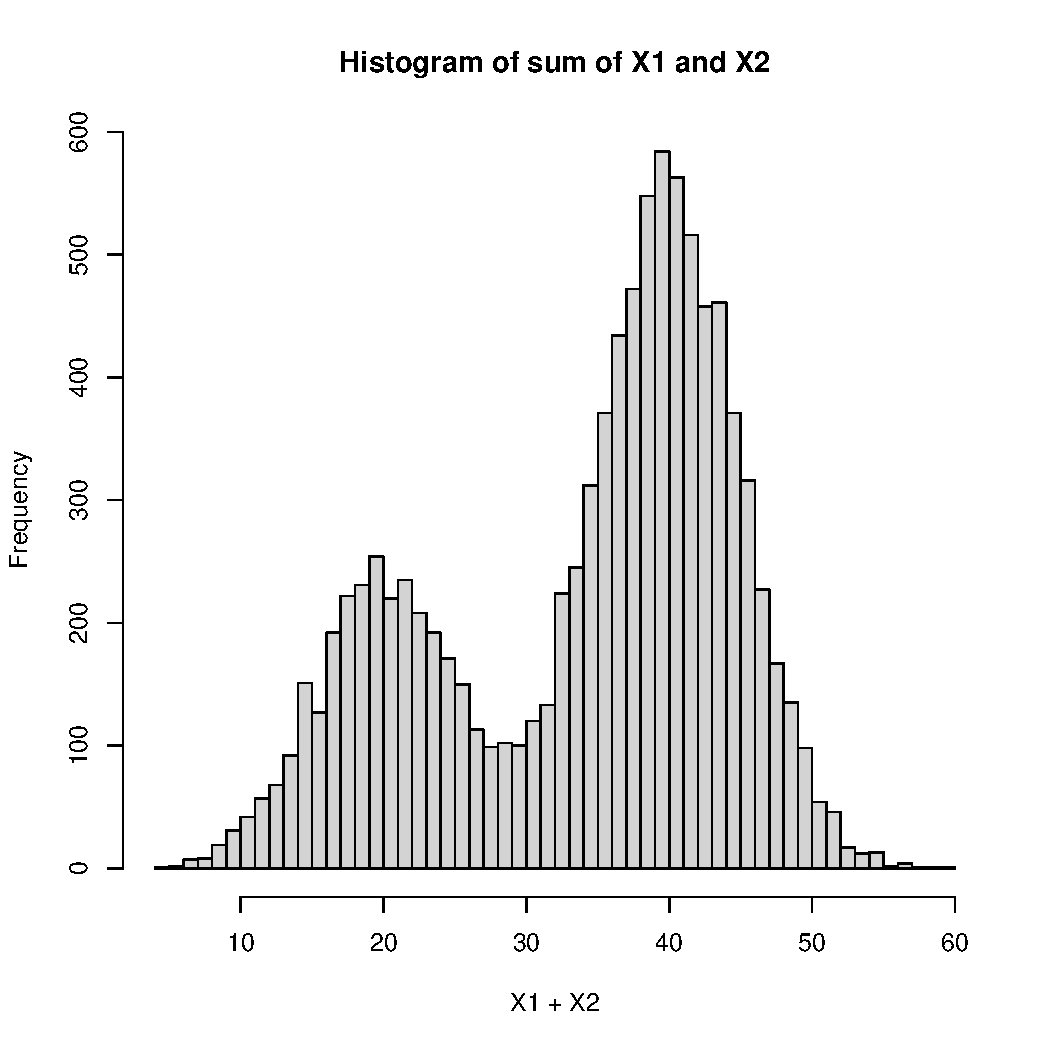
\includegraphics[width=\maxwidth]{figure/unnamed-chunk-3-1} 

}


\end{knitrout}
We can then obtain the estimated values for $\pi_i, \boldmu_i$ and $\boldSigma_i$:
\begin{knitrout}
\definecolor{shadecolor}{rgb}{0.969, 0.969, 0.969}\color{fgcolor}\begin{kframe}
\begin{alltt}
  \hlstd{EMmixtool[}\hlkwd{c}\hlstd{(}\hlstr{"lambda"}\hlstd{,} \hlstr{"mu"}\hlstd{,} \hlstr{"sigma"}\hlstd{)]}
\end{alltt}
\begin{verbatim}
## $lambda
## [1] 0.2994075 0.7005925
## 
## $mu
## [1] 20.03593 39.95081
## 
## $sigma
## [1] 4.932609 5.003639
\end{verbatim}
\end{kframe}
\end{knitrout}

Now we will execute the EM algorithm by hand and compare it to the values found by \texttt{normalmixEM()}. For this, we first inspect the histogram above which shows us two distinct peaks. This suggests that there are two major clusters and suggests using $k$-means with 2 clusters. We then store the means, standard deviations and mixture components:\\

\begin{knitrout}
\definecolor{shadecolor}{rgb}{0.969, 0.969, 0.969}\color{fgcolor}\begin{kframe}
\begin{alltt}
\hlstd{mem} \hlkwb{<-} \hlkwd{kmeans}\hlstd{(x,}\hlnum{2}\hlstd{)}\hlopt{$}\hlstd{cluster}
\hlstd{mu1} \hlkwb{<-} \hlkwd{mean}\hlstd{(x[mem}\hlopt{==}\hlnum{1}\hlstd{])}
\hlstd{mu2} \hlkwb{<-} \hlkwd{mean}\hlstd{(x[mem}\hlopt{==}\hlnum{2}\hlstd{])}
\hlstd{sigma1} \hlkwb{<-} \hlkwd{sd}\hlstd{(x[mem}\hlopt{==}\hlnum{1}\hlstd{])}
\hlstd{sigma2} \hlkwb{<-} \hlkwd{sd}\hlstd{(x[mem}\hlopt{==}\hlnum{2}\hlstd{])}
\hlstd{pi1} \hlkwb{<-} \hlkwd{sum}\hlstd{(mem}\hlopt{==}\hlnum{1}\hlstd{)}\hlopt{/}\hlkwd{length}\hlstd{(mem)}
\hlstd{pi2} \hlkwb{<-} \hlkwd{sum}\hlstd{(mem}\hlopt{==}\hlnum{2}\hlstd{)}\hlopt{/}\hlkwd{length}\hlstd{(mem)}
\end{alltt}
\end{kframe}
\end{knitrout}
We employ the method \texttt{sum.finite()} to omit any infinite values of $x$ that may arise:
\begin{knitrout}
\definecolor{shadecolor}{rgb}{0.969, 0.969, 0.969}\color{fgcolor}\begin{kframe}
\begin{alltt}
\hlcom{# modified sum only considers finite values}
\hlstd{sum.finite} \hlkwb{<-} \hlkwa{function}\hlstd{(}\hlkwc{x}\hlstd{) \{}
  \hlkwd{sum}\hlstd{(x[}\hlkwd{is.finite}\hlstd{(x)])}
\hlstd{\}}
\end{alltt}
\end{kframe}
\end{knitrout}
Subsequently, we calculate the initial value of $Q(\boldPsi; \boldPsi^{(k)})$ by plugging into the right hand side of \eqref{eq:EMFirstStep}: \\
\begin{knitrout}
\definecolor{shadecolor}{rgb}{0.969, 0.969, 0.969}\color{fgcolor}\begin{kframe}
\begin{alltt}
\hlstd{Q} \hlkwb{<-} \hlnum{0}
\hlcom{# starting value of expected value of the log likelihood}
\hlstd{Q[}\hlnum{2}\hlstd{]} \hlkwb{<-} \hlkwd{sum.finite}\hlstd{(}\hlkwd{log}\hlstd{(pi1)}\hlopt{+}\hlkwd{log}\hlstd{(}\hlkwd{dnorm}\hlstd{(x, mu1, sigma1)))}
  \hlopt{+} \hlkwd{sum.finite}\hlstd{(}\hlkwd{log}\hlstd{(pi2)}\hlopt{+}\hlkwd{log}\hlstd{(}\hlkwd{dnorm}\hlstd{(x, mu2, sigma2)))}
\end{alltt}
\begin{verbatim}
## [1] -95411.23
\end{verbatim}
\end{kframe}
\end{knitrout}


We closely follow the Gaussian version of the EM algorithm as in \hyperref[sec:GMMs]{Section 3}, paying attention to equations \eqref{eq:EStepGMM} for the E-step and \eqref{eq:Mstep2GMM} for the M-step: \\
\begin{knitrout}
\definecolor{shadecolor}{rgb}{0.969, 0.969, 0.969}\color{fgcolor}\begin{kframe}
\begin{alltt}
\hlstd{k} \hlkwb{<-} \hlnum{2}

\hlkwa{while} \hlstd{(}\hlkwd{abs}\hlstd{(Q[k]}\hlopt{-}\hlstd{Q[k}\hlopt{-}\hlnum{1}\hlstd{])}\hlopt{>=}\hlnum{1e-6}\hlstd{) \{}
  \hlcom{# E step}
  \hlstd{comp1} \hlkwb{<-} \hlstd{pi1} \hlopt{*} \hlkwd{dnorm}\hlstd{(x, mu1, sigma1)}
  \hlstd{comp2} \hlkwb{<-} \hlstd{pi2} \hlopt{*} \hlkwd{dnorm}\hlstd{(x, mu2, sigma2)}
  \hlstd{comp.sum} \hlkwb{<-} \hlstd{comp1} \hlopt{+} \hlstd{comp2}

  \hlstd{p1} \hlkwb{<-} \hlstd{comp1}\hlopt{/}\hlstd{comp.sum}
  \hlstd{p2} \hlkwb{<-} \hlstd{comp2}\hlopt{/}\hlstd{comp.sum}

  \hlcom{# M step}
  \hlstd{pi1} \hlkwb{<-} \hlkwd{sum.finite}\hlstd{(p1)} \hlopt{/} \hlkwd{length}\hlstd{(x)}
  \hlstd{pi2} \hlkwb{<-} \hlkwd{sum.finite}\hlstd{(p2)} \hlopt{/} \hlkwd{length}\hlstd{(x)}

  \hlstd{mu1} \hlkwb{<-} \hlkwd{sum.finite}\hlstd{(p1} \hlopt{*} \hlstd{x)} \hlopt{/} \hlkwd{sum.finite}\hlstd{(p1)}
  \hlstd{mu2} \hlkwb{<-} \hlkwd{sum.finite}\hlstd{(p2} \hlopt{*} \hlstd{x)} \hlopt{/} \hlkwd{sum.finite}\hlstd{(p2)}

  \hlstd{sigma1} \hlkwb{<-} \hlkwd{sqrt}\hlstd{(}\hlkwd{sum.finite}\hlstd{(p1} \hlopt{*} \hlstd{(x}\hlopt{-}\hlstd{mu1)}\hlopt{^}\hlnum{2}\hlstd{)} \hlopt{/} \hlkwd{sum.finite}\hlstd{(p1))}
  \hlstd{sigma2} \hlkwb{<-} \hlkwd{sqrt}\hlstd{(}\hlkwd{sum.finite}\hlstd{(p2} \hlopt{*} \hlstd{(x}\hlopt{-}\hlstd{mu2)}\hlopt{^}\hlnum{2}\hlstd{)} \hlopt{/} \hlkwd{sum.finite}\hlstd{(p2))}

  \hlstd{p1} \hlkwb{<-} \hlstd{pi1}
  \hlstd{p2} \hlkwb{<-} \hlstd{pi2}

  \hlstd{k} \hlkwb{<-} \hlstd{k} \hlopt{+} \hlnum{1}
  \hlstd{Q[k]} \hlkwb{<-} \hlkwd{sum}\hlstd{(}\hlkwd{log}\hlstd{(comp.sum))}
\hlstd{\}}
\end{alltt}
\end{kframe}
\end{knitrout}
Comparing our results done ``by hand'' with the one from \texttt{normalmixEM}, our results align with the \texttt{mixtools} package:\\
\begin{knitrout}
\definecolor{shadecolor}{rgb}{0.969, 0.969, 0.969}\color{fgcolor}\begin{kframe}
\begin{alltt}
  \hlstd{EMmixtool[}\hlstr{"lambda"}\hlstd{]}
\end{alltt}
\begin{verbatim}
## $lambda
## [1] 0.2994075 0.7005925
\end{verbatim}
\begin{alltt}
  \hlkwd{c}\hlstd{(pi2, pi1)}
\end{alltt}
\begin{verbatim}
## [1] 0.2994099 0.7005901
\end{verbatim}
\begin{alltt}
  \hlstd{EMmixtool[}\hlstr{"mu"}\hlstd{]}
\end{alltt}
\begin{verbatim}
## $mu
## [1] 20.03593 39.95081
\end{verbatim}
\begin{alltt}
  \hlkwd{c}\hlstd{(mu2, mu1)}
\end{alltt}
\begin{verbatim}
## [1] 20.03600 39.95084
\end{verbatim}
\begin{alltt}
  \hlstd{EMmixtool[}\hlstr{"sigma"}\hlstd{]}
\end{alltt}
\begin{verbatim}
## $sigma
## [1] 4.932609 5.003639
\end{verbatim}
\begin{alltt}
  \hlkwd{c}\hlstd{(sigma2, sigma1)}
\end{alltt}
\begin{verbatim}
## [1] 4.932672 5.003607
\end{verbatim}
\end{kframe}
\end{knitrout}

\subsection{Iris Dataset with GMMs}
Based on the python code from \cite{Iris_Implementation}.

We now turn to a more practical example using the Iris dataset \cite{Dua:2019}. The data set consists of 50 samples from three species of the flower Iris. Four features: the lengths and widths of the sepals and petals were measured for each sample. It is one of the most commonly used datasets for basic statistical analysis.

We begin in a similar fashion to the previous example by importing \texttt{mixtools}, a new package \texttt{factoextra} as well as the Iris dataset itself.
\singlespacing
\begin{knitrout}
\definecolor{shadecolor}{rgb}{0.969, 0.969, 0.969}\color{fgcolor}\begin{kframe}
\begin{alltt}
  \hlcom{# Import packages and general graph setup}
  \hlkwd{suppressPackageStartupMessages}\hlstd{(}\hlkwd{library}\hlstd{(factoextra))}
  \hlkwd{suppressPackageStartupMessages}\hlstd{(}\hlkwd{library}\hlstd{(mixtools))}
  \hlkwd{data}\hlstd{(iris)}
  \hlkwd{par}\hlstd{(}\hlkwc{mfrow}\hlstd{=}\hlkwd{c}\hlstd{(}\hlnum{1}\hlstd{,}\hlnum{2}\hlstd{))}
  \hlkwd{set.seed}\hlstd{(}\hlnum{1234}\hlstd{)}
\end{alltt}
\end{kframe}
\end{knitrout}

For this example, we will only consider the two features ``Petal.Length'' and ``Petal.Width''. We then perform $k$--means, knowing a priori that there will be three clusters involved. We use the method \texttt{fviz\_cluster()} from \texttt{factoextra} to visualise the clusters at hand. \\

\begin{knitrout}
\definecolor{shadecolor}{rgb}{0.969, 0.969, 0.969}\color{fgcolor}\begin{kframe}
\begin{alltt}
  \hlstd{iris.nolabel} \hlkwb{=} \hlstd{iris[,}\hlnum{3}\hlopt{:}\hlnum{4}\hlstd{]}
  \hlstd{k1} \hlkwb{<-} \hlkwd{kmeans}\hlstd{(}\hlkwc{x}\hlstd{=iris.nolabel,} \hlkwc{centers}\hlstd{=}\hlnum{3}\hlstd{)}
  \hlkwd{fviz_cluster}\hlstd{(k1,} \hlkwc{data}\hlstd{=iris.nolabel)}
\end{alltt}
\end{kframe}

{\centering \includegraphics[width=4in]{figure/unnamed-chunk-11-1} 

}


\end{knitrout}

This time, however, running the multivariate normal EM algorithm, we run into a very inaccurate plot. The centers are classified far worse than $k$-means and each category overlaps each other extensively. \\ 

\begin{knitrout}
\definecolor{shadecolor}{rgb}{0.969, 0.969, 0.969}\color{fgcolor}\begin{kframe}
\begin{alltt}
  \hlstd{irisEM} \hlkwb{<-} \hlkwd{mvnormalmixEM}\hlstd{(iris.nolabel,} \hlkwc{k}\hlstd{=}\hlnum{3}\hlstd{)}
\end{alltt}
\begin{verbatim}
## number of iterations= 89
\end{verbatim}
\begin{alltt}
  \hlkwd{suppressWarnings}\hlstd{(}\hlkwd{summary}\hlstd{(irisEM))}
\end{alltt}
\begin{verbatim}
## summary of mvnormalmixEM object:
##          comp 1   comp 2
## lambda 0.348627 0.330089
## mu1    5.019893 1.862490
## mu2    1.460476 0.242997
## mu3    4.749200 1.462283
## loglik at estimate:  -134.1357
\end{verbatim}
\begin{alltt}
  \hlkwd{par}\hlstd{(}\hlkwc{mfrow}\hlstd{=}\hlkwd{c}\hlstd{(}\hlnum{1}\hlstd{,}\hlnum{2}\hlstd{))}
  \hlkwd{plot}\hlstd{(irisEM,} \hlkwc{density}\hlstd{=}\hlnum{TRUE}\hlstd{)}
\end{alltt}
\end{kframe}

{\centering \includegraphics[width=\maxwidth]{figure/unnamed-chunk-12-1} 

}


\end{knitrout}

As mentioned in \hyperref[subsec:start]{Subsection 2.3}, this issue is likely cause by poor starting values. Using a similar approach to the first example, we would like to use $k$-means to then find better initial estimates for the parameter vector $\boldtheta_i$. This time, we must consider that our data is multivariate. \\
\begin{knitrout}
\definecolor{shadecolor}{rgb}{0.969, 0.969, 0.969}\color{fgcolor}\begin{kframe}
\begin{alltt}
  \hlstd{mem} \hlkwb{<-} \hlstd{k1}\hlopt{$}\hlstd{cluster}

  \hlstd{pi1iris} \hlkwb{<-} \hlstd{k1}\hlopt{$}\hlstd{size[}\hlnum{1}\hlstd{]}\hlopt{/}\hlkwd{length}\hlstd{(mem)}
  \hlstd{pi2iris} \hlkwb{<-} \hlstd{k1}\hlopt{$}\hlstd{size[}\hlnum{2}\hlstd{]}\hlopt{/}\hlkwd{length}\hlstd{(mem)}
  \hlstd{pi3iris} \hlkwb{<-} \hlstd{k1}\hlopt{$}\hlstd{size[}\hlnum{3}\hlstd{]}\hlopt{/}\hlkwd{length}\hlstd{(mem)}

  \hlstd{mu1iris} \hlkwb{<-} \hlstd{k1}\hlopt{$}\hlstd{centers[}\hlnum{1}\hlstd{,]}
  \hlstd{mu2iris} \hlkwb{<-} \hlstd{k1}\hlopt{$}\hlstd{centers[}\hlnum{2}\hlstd{,]}
  \hlstd{mu3iris} \hlkwb{<-} \hlstd{k1}\hlopt{$}\hlstd{centers[}\hlnum{3}\hlstd{,]}

  \hlstd{sigma1iris} \hlkwb{<-} \hlkwd{diag}\hlstd{(}\hlkwd{c}\hlstd{(}\hlkwd{sd}\hlstd{(iris.nolabel[mem}\hlopt{==}\hlnum{1}\hlstd{,}\hlnum{1}\hlstd{]),} \hlkwd{sd}\hlstd{(iris.nolabel[mem}\hlopt{==}\hlnum{1}\hlstd{,}\hlnum{2}\hlstd{])))}
  \hlstd{sigma2iris} \hlkwb{<-} \hlkwd{diag}\hlstd{(}\hlkwd{c}\hlstd{(}\hlkwd{sd}\hlstd{(iris.nolabel[mem}\hlopt{==}\hlnum{2}\hlstd{,}\hlnum{1}\hlstd{]),} \hlkwd{sd}\hlstd{(iris.nolabel[mem}\hlopt{==}\hlnum{2}\hlstd{,}\hlnum{2}\hlstd{])))}
  \hlstd{sigma3iris} \hlkwb{<-} \hlkwd{diag}\hlstd{(}\hlkwd{c}\hlstd{(}\hlkwd{sd}\hlstd{(iris.nolabel[mem}\hlopt{==}\hlnum{3}\hlstd{,}\hlnum{1}\hlstd{]),} \hlkwd{sd}\hlstd{(iris.nolabel[mem}\hlopt{==}\hlnum{3}\hlstd{,}\hlnum{2}\hlstd{])))}
\end{alltt}
\end{kframe}
\end{knitrout}

Running \texttt{mvnormalmixEM()} again, we obtain a much improved estimation using the EM algorithm: \\
\begin{knitrout}
\definecolor{shadecolor}{rgb}{0.969, 0.969, 0.969}\color{fgcolor}\begin{kframe}
\begin{alltt}
  \hlstd{irisEM2} \hlkwb{<-} \hlkwd{mvnormalmixEM}\hlstd{(iris.nolabel,} \hlkwc{lambda}\hlstd{=}\hlkwd{c}\hlstd{(pi1iris, pi2iris, pi3iris),}
                         \hlkwc{mu}\hlstd{=}\hlkwd{list}\hlstd{(mu1iris, mu2iris, mu3iris),}
                         \hlkwc{sigma}\hlstd{=}\hlkwd{list}\hlstd{(sigma1iris, sigma2iris, sigma3iris),} \hlkwc{k}\hlstd{=}\hlnum{3}\hlstd{)}
\end{alltt}
\begin{verbatim}
## number of iterations= 87
\end{verbatim}
\begin{alltt}
  \hlkwd{par}\hlstd{(}\hlkwc{mfrow}\hlstd{=}\hlkwd{c}\hlstd{(}\hlnum{1}\hlstd{,}\hlnum{2}\hlstd{))}
  \hlkwd{plot}\hlstd{(irisEM2,} \hlkwc{density}\hlstd{=}\hlnum{TRUE}\hlstd{)}
\end{alltt}
\end{kframe}

{\centering \includegraphics[width=\maxwidth]{figure/unnamed-chunk-14-1} 

}


\end{knitrout}

The coefficient estimates are as follows: \\
\begin{knitrout}
\definecolor{shadecolor}{rgb}{0.969, 0.969, 0.969}\color{fgcolor}\begin{kframe}
\begin{alltt}
  \hlstd{irisEM2}\hlopt{$}\hlstd{lambda}
\end{alltt}
\begin{verbatim}
## [1] 0.3333329 0.3410062 0.3256608
\end{verbatim}
\begin{alltt}
  \hlstd{irisEM2}\hlopt{$}\hlstd{mu}
\end{alltt}
\begin{verbatim}
## [[1]]
## [1] 1.4619996 0.2459998
## 
## [[2]]
## [1] 4.287863 1.335230
## 
## [[3]]
## [1] 5.553260 2.032826
\end{verbatim}
\begin{alltt}
  \hlstd{irisEM2}\hlopt{$}\hlstd{sigma}
\end{alltt}
\begin{verbatim}
## [[1]]
##            [,1]       [,2]
## [1,] 0.02955588 0.00594794
## [2,] 0.00594794 0.01088395
## 
## [[2]]
##            [,1]       [,2]
## [1,] 0.24167567 0.07951146
## [2,] 0.07951146 0.04148781
## 
## [[3]]
##            [,1]       [,2]
## [1,] 0.30922741 0.05037616
## [2,] 0.05037616 0.07330311
\end{verbatim}
\end{kframe}
\end{knitrout}
\newpage
\printbibliography
 
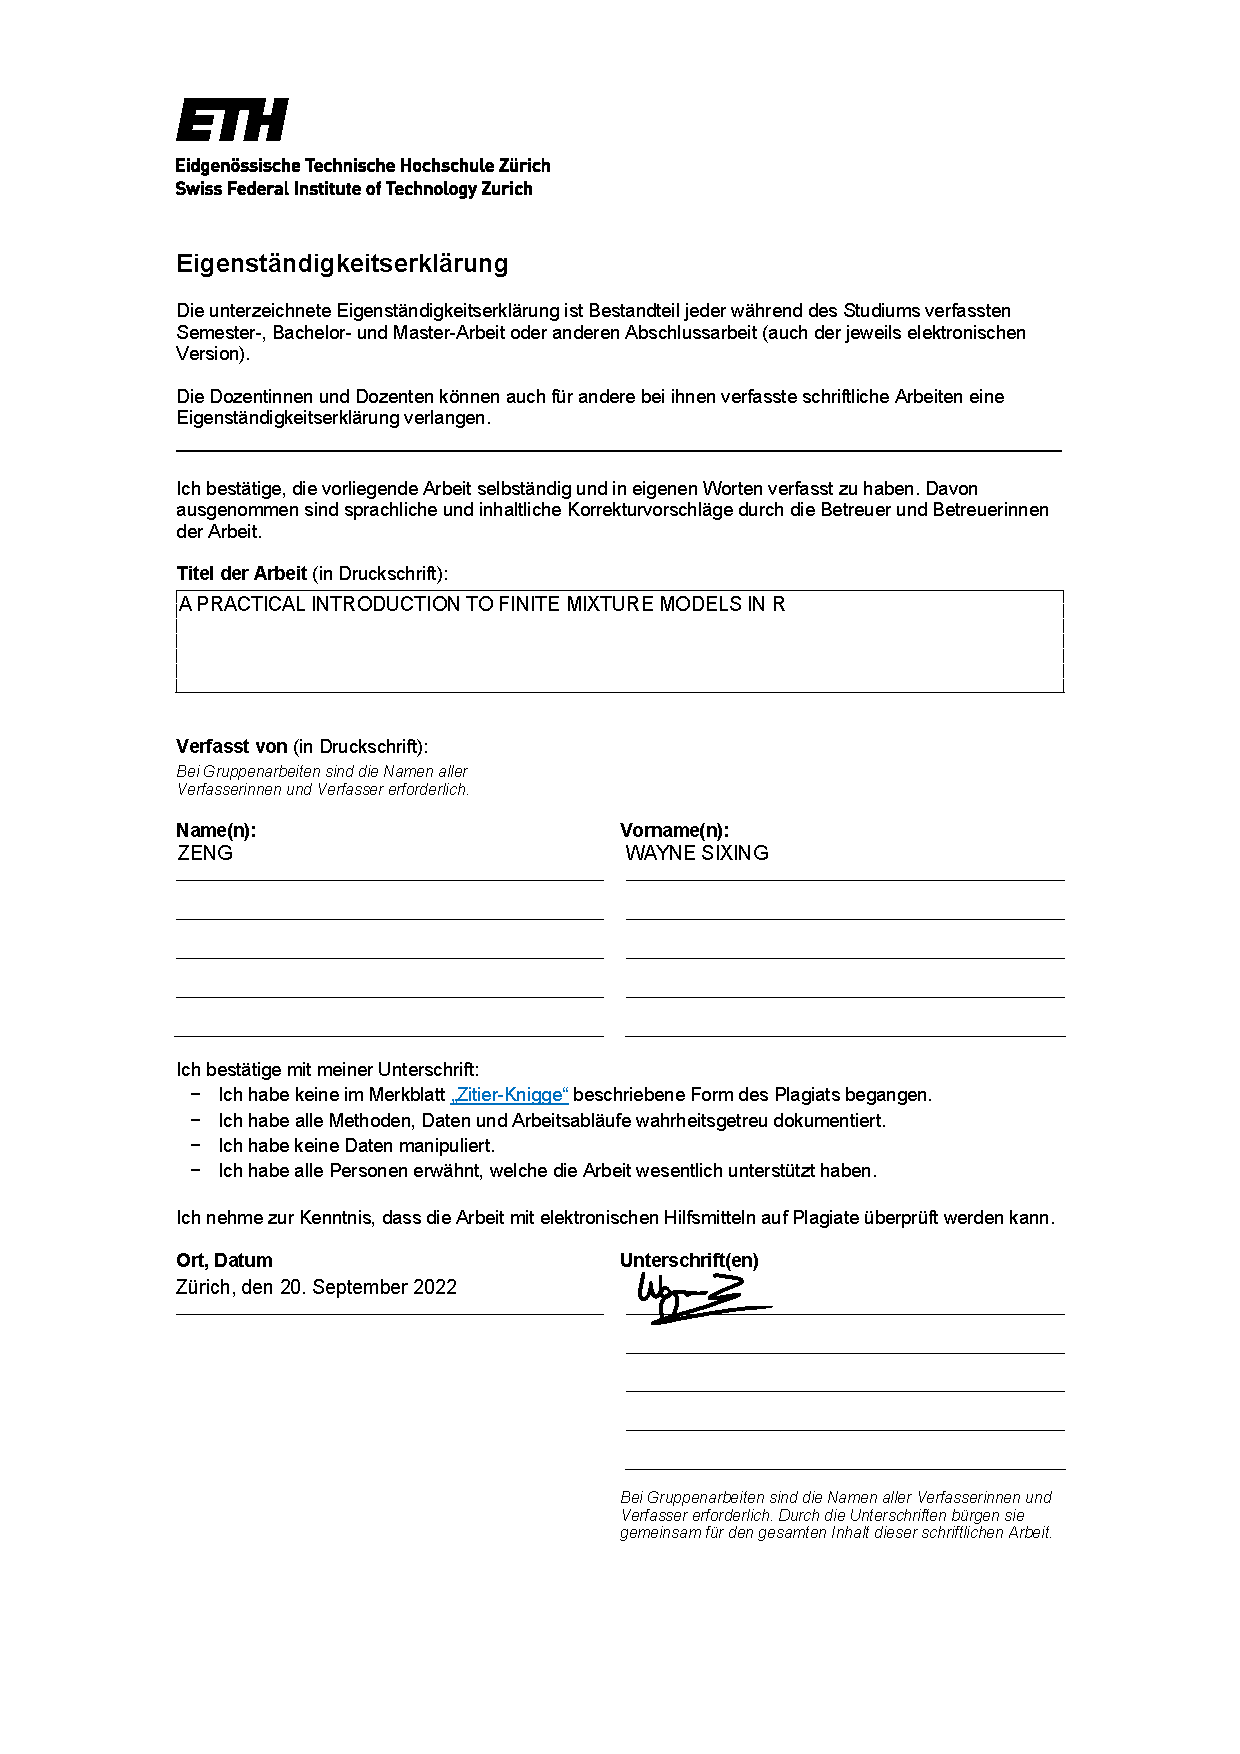
\includepdf[pages=-]{images/declaration_fmm.pdf}
\end{document}
